\chapter{Binaire diagrammen vast-vloeibaar}\label{ch:b2:solid-liquid-diagrams}

Tin smelt bij \qty{232}{\degreeCelsius} en lood bij \qty{327}{\degreeCelsius},
en toch smelt het oude soldeer van elektriciens, een mengsel van de twee, bij
\qty{182}{\degreeCelsius}, onder beide. Zout dat op een weg gestrooid wordt, smelt ijs, maar slechts
tot ongeveer \qty{-21}{\degreeCelsius}; in een koudere nacht doet het niets.
Koper en nikkel daarentegen mengen in elke verhouding, zelfs in de
vaste toestand, en hun legeringen smelten over een temperatuurgebied tussen dat van de
twee metalen. De diagrammen van dit hoofdstuk zeggen voor elk paar welke vaste stoffen
uit een afkoelende vloeistof kristalliseren, bij welke temperaturen en in welke
hoeveelheden --- de kennis achter elk gietstuk, elke soldeerverbinding en elke
laagsmeltende legering.

\begin{recall}
\Cref{ch:b2:chemical-potential}: \omterm{def:b2:chemical-potential:chemical-potential}{chemische potentiaal} van een bestanddeel in een \omterm{def:b2:chemical-potential:ideal-mixture}{ideaal
mengsel}, cryoscopie. \Cref{ch:b2:equilibrium-shifts}: de \omterm{def:b2:equilibrium-shifts:variance}{variantie}.
\Cref{ch:b2:liquid-vapour-diagrams}: \omterm{def:b2:liquid-vapour-diagrams:binary-diagram}{binaire diagrammen}, verbindingslijnen en de
\omterm{thm:b2:liquid-vapour-diagrams:lever}{hefboomregel}. Het deel van jaar~1: metaalbinding, substitutie- en interstitiële
legeringen, kristaltypen.
\end{recall}

\begin{omfigure}
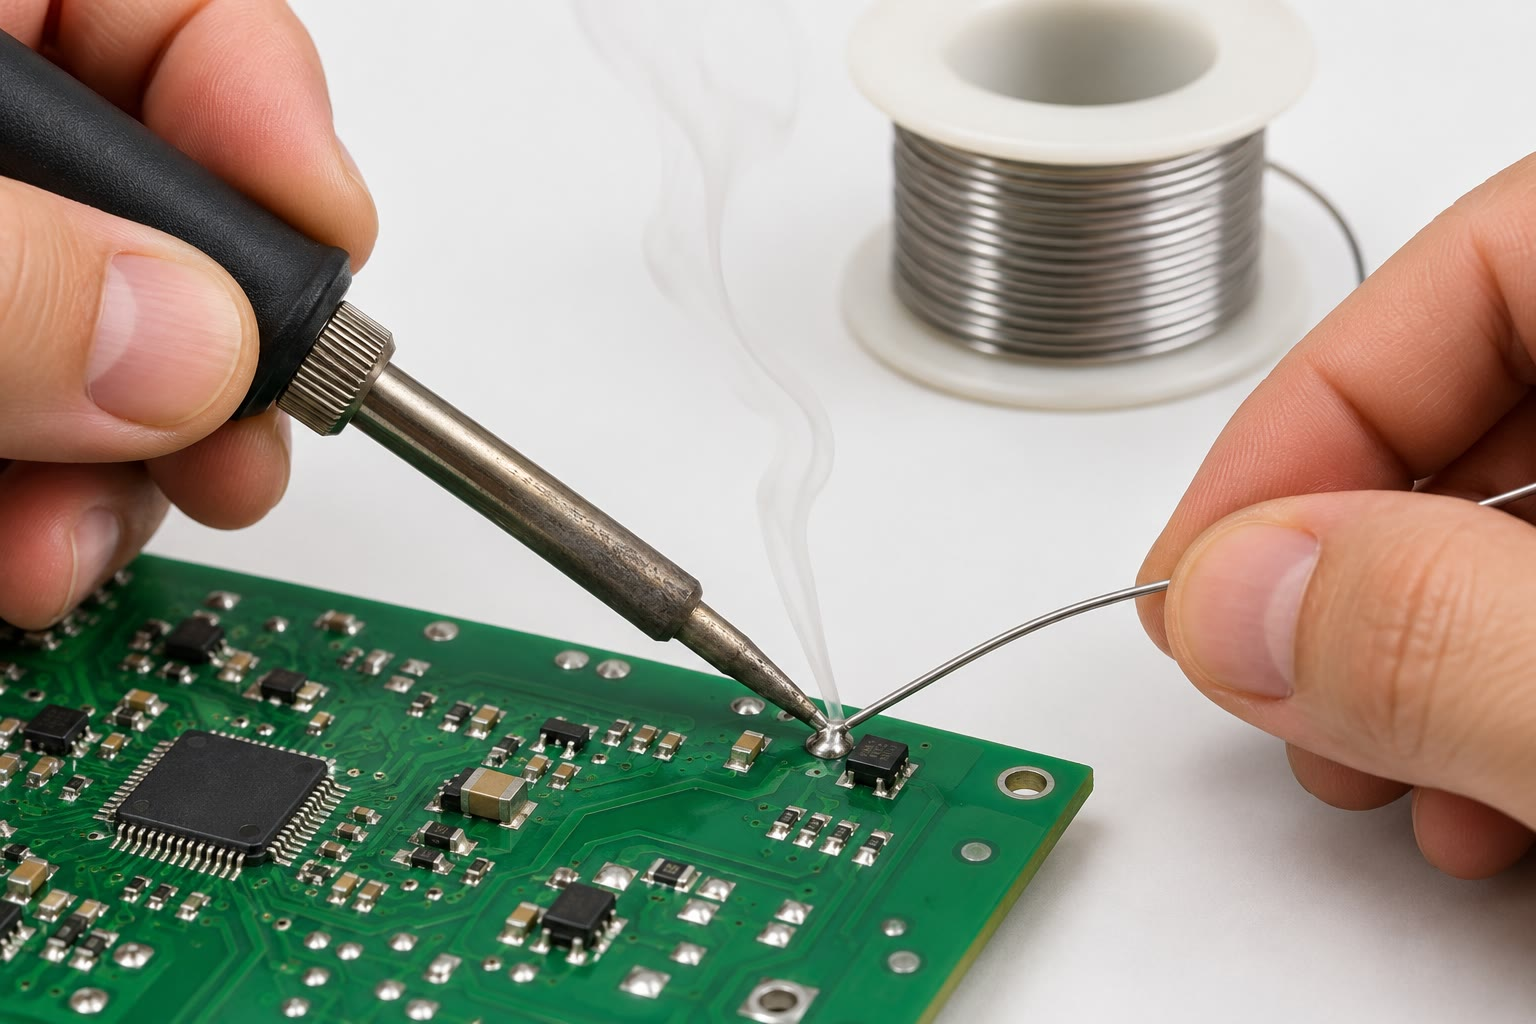
\includegraphics[width=0.6\linewidth]{images/book3/ai/b2-08-soldering.jpg}

{\small Een component op een printplaat solderen: de soldeerdraad smelt bij
contact met de hete bout en de verbinding stolt binnen een seconde wanneer de bout
wordt opgetild --- omdat de legering bij één enkele, lage temperatuur smelt.}
\end{omfigure}

\section{Thermische analyse}

\begin{definition}[Thermische analyse]\label{def:b2:solid-liquid-diagrams:cooling-curve}
\emph{Thermische analyse}\index{thermische analyse} bepaalt de temperaturen van
de faseovergangen van een monster uit zijn temperatuur, geregistreerd terwijl het
met een constante snelheid wordt verwarmd of afgekoeld. De registratie van de temperatuur als functie van de tijd
tijdens een langzame afkoeling is een \emph{afkoelingskromme}\index{afkoelingskromme}.
\end{definition}

Ver van elke faseovergang koelt het monster gelijkmatig af. Wanneer een vaste stof begint te
kristalliseren, vertraagt de kristallisatiewarmte de afkoeling: de kromme vertoont een
knik, of blijft een tijd op een constante temperatuur staan --- een
\textit{plateau} --- als het stollen bij vaste temperatuur gebeurt.

\begin{proposition}[Plateaus]\label{prop:b2:solid-liquid-diagrams:plateaus}
Bij vaste druk stolt een zuivere stof bij constante temperatuur, en dat
doet ook een binaire vloeistof waaruit twee vaste stoffen samen kristalliseren. Een binaire
vloeistof waaruit één vaste stof kristalliseert, stolt over een temperatuurgebied.
\end{proposition}

\begin{proof}
Bij vaste druk is de \omterm{def:b2:equilibrium-shifts:variance}{variantie} $v = n - r + 1 - \varphi$. Zuivere
stof, vloeistof + vaste stof: $v = 1 + 1 - 2 = 0$. Binair, vloeistof + twee vaste stoffen:
$v = 2 + 1 - 3 = 0$. Binair, vloeistof + één vaste stof: $v = 2 + 1 - 2 = 1$: de
temperatuur verandert mee met de samenstelling van de vloeistof. Een \omterm{def:b2:equilibrium-shifts:variance}{variantie} 0 betekent dat de
temperatuur niet kan veranderen zolang alle fasen aanwezig zijn: de afgevoerde warmte wordt
geleverd door het stollen, tot een fase verdwijnt.
\end{proof}

\begin{omfigure}
\begin{tikzpicture}[font=\small, x=0.55cm, y=0.05cm]
  \foreach \dx/\name in {0/zuiver metaal, 9/{mengsel, eerst één vaste stof}, 18/eutectisch mengsel} {
    \draw[->] (\dx,0) -- (\dx+7.5,0) node[below left, font=\scriptsize] {$t$};
    \draw[->] (\dx,0) -- (\dx,62) node[above, font=\scriptsize] {$T$};
    \node[font=\scriptsize] at (\dx+3.8,-8) {\name};
  }
  % pure: cool, plateau at 40, cool
  \draw[omDef, thick] (0,58) .. controls (1,48) and (1.6,42) .. (2,40) -- (4.5,40) .. controls (5.2,32) and (6,24) .. (7,20);
  \node[font=\scriptsize, anchor=south] at (3.25,40.5) {plateau};
  % mixture: cool, break at 48, slow fall, plateau at 30, cool
  \draw[omDef, thick] (9,58) .. controls (9.6,53) and (9.9,50) .. (10.2,48)
     .. controls (11,42) and (11.6,35) .. (12.3,30) -- (14.2,30) .. controls (14.9,23) and (15.6,17) .. (16.5,14);
  \node[font=\scriptsize, anchor=west] at (10.4,49.5) {knik};
  \node[font=\scriptsize, anchor=south] at (13.25,30.5) {eutecticum};
  % eutectic: plateau at 30
  \draw[omDef, thick] (18,58) .. controls (19,46) and (19.8,36) .. (20.5,30) -- (24,30) .. controls (24.7,23) and (25.4,17) .. (26.2,14);
  \node[font=\scriptsize, anchor=south] at (22.25,30.5) {plateau};
\end{tikzpicture}

{\small \omterm{def:b2:solid-liquid-diagrams:cooling-curve}{Afkoelingskrommen}, schematisch. Een zuiver metaal stolt op een plateau. Een
mengsel vertoont een knik wanneer de eerste vaste stof verschijnt, daarna de langzame
afkoeling van een vloeistof die over een temperatuurgebied stolt, en dan het
plateau van het eutecticum. Een vloeistof met de eutectische samenstelling stolt op één
enkel plateau, zoals een zuivere stof.}
\end{omfigure}

\begin{method}[Een diagram opbouwen uit afkoelingskrommen]\label{met:b2:solid-liquid-diagrams:diagram-from-curves}
\begin{enumerate}
  \item Registreer \omterm{def:b2:solid-liquid-diagrams:cooling-curve}{afkoelingskrommen} voor een reeks samenstellingen, de zuivere bestanddelen
        inbegrepen.
  \item Zet in een grafiek (samenstelling, temperatuur) voor elke samenstelling de
        temperatuur uit van de eerste knik (het begin van de kristallisatie) en van
        elk plateau.
  \item Verbind de punten van eerste kristallisatie: dat is de \omterm{def:b2:solid-liquid-diagrams:liquidus}{liquidus}. Verbind
        de einden van het stollen: de \omterm{def:b2:solid-liquid-diagrams:liquidus}{solidus}. Een plateau dat bij veel samenstellingen op dezelfde
        temperatuur gevonden wordt, is een invariante lijn (een eutecticum).
  \item De lengte van het eutectische plateau, het grootst bij de eutectische
        samenstelling, lokaliseert die samenstelling.
\end{enumerate}
\end{method}

\section{Volledige mengbaarheid in de vaste toestand}

\begin{definition}[Vaste oplossing]\label{def:b2:solid-liquid-diagrams:solid-solution}
Een \emph{vaste oplossing}\index{vaste oplossing} is één enkele kristallijne fase met
variabele samenstelling, waarin atomen van het ene bestanddeel atomen van het
andere vervangen op de roosterplaatsen van hetzelfde rooster (substitutie) of de holten van
dat rooster bezetten (interstitieel).
\end{definition}

Koper en nikkel hebben dezelfde kubisch vlakgecentreerde structuur en atomen met
vergelijkbare stralen: ze vormen bij elke samenstelling een vaste substitutieoplossing.

\begin{definition}[Liquidus en solidus]\label{def:b2:solid-liquid-diagrams:liquidus}
In een diagram vast-vloeibaar is de \emph{liquidus}\index{liquidus} de kromme
waarboven alles vloeibaar is; ze geeft de samenstelling van de vloeistof in
evenwicht met een vaste stof. De \emph{solidus}\index{solidus} is de kromme waaronder
alles vast is; waar de vaste stof een oplossing is, geeft ze de
samenstelling van de vaste stof in evenwicht met de vloeistof.
\end{definition}

\begin{proposition}[De lens]\label{prop:b2:solid-liquid-diagrams:lens}
Als de twee bestanddelen ideale oplossingen vormen in de vloeistof en in de vaste stof,
verbinden de \omterm{def:b2:solid-liquid-diagrams:liquidus}{liquidus} en de \omterm{def:b2:solid-liquid-diagrams:liquidus}{solidus} de twee smeltpunten en omsluiten ze een
lensvormig tweefasengebied; bij elke temperatuur zijn de molfracties $x_i$ van
elk bestanddeel in de vloeistof en in de vaste stof verbonden door
\[
  \frac{x_i^{\ell}}{x_i^{s}} = \exp\left[-\frac{\Delta_{\text{fus}}H_i}{R}\left(\frac1T - \frac1{T_i^*}\right)\right] .
\]
\end{proposition}

\begin{proof}
De \omterm{def:b2:chemical-potential:chemical-potential}{chemische potentiaal} van $i$ is dezelfde in beide fasen, $\mu_i^{*,s} +
RT\ln x_i^s = \mu_i^{*,\ell} + RT\ln x_i^\ell$, dus $RT\ln(x_i^\ell/x_i^s) =
-(\mu_i^{*,\ell} - \mu_i^{*,s}) = -\Delta_{\text{fus}}G_i(T)$, en met constante
$\Delta_{\text{fus}}H_i$ is $\Delta_{\text{fus}}G_i = \Delta_{\text{fus}}H_i(1 - T/T_i^*)$.
Samen met $x_1 + x_2 = 1$ in elke fase leggen de twee betrekkingen de twee
samenstellingen bij elke $T$ vast (numeriek opgelost voor de figuur); dat de
resulterende krommen een lens vormen, wordt aangenomen.
\end{proof}

\begin{omfigure}
\begin{tikzpicture}
\begin{axis}[omphase, width=0.62\linewidth, height=7cm, ymin=1050, ymax=1480,
  xlabel={$x$ (nikkel)}, ylabel={$T$ (\unit{\degreeCelsius})}]
\addplot[omliquidus] table[x=xl, y=T] {figdata/out/bachelor-2-solid-liquid-a.dat};
\addplot[omsolidus] table[x=xs, y=T] {figdata/out/bachelor-2-solid-liquid-a.dat};
\draw[tieline] (axis cs:0.541,1300) -- (axis cs:0.609,1300);
\fill (axis cs:0.58,1300) circle (1.3pt);
\node[font=\scriptsize] at (axis cs:0.25,1400) {vloeistof};
\node[font=\scriptsize] at (axis cs:0.8,1150) {vaste oplossing};
\node[font=\scriptsize, anchor=east] at (axis cs:0.5,1330) {liquidus};
\node[font=\scriptsize, anchor=west] at (axis cs:0.66,1290) {solidus};
\node[font=\scriptsize, anchor=west] at (axis cs:0.03,1080) {\qty{1085}{\degreeCelsius}};
\draw[black!50] (axis cs:0.005,1084) -- (axis cs:0.03,1080);
\node[font=\scriptsize, anchor=south east] at (axis cs:1.0,1456) {\qty{1455}{\degreeCelsius}};
\end{axis}
\end{tikzpicture}

{\small Koper--nikkel, berekend voor ideale vaste en vloeibare oplossingen uit de
smeltpunten en smeltenthalpieën van de twee metalen. Bij
\qty{1300}{\degreeCelsius} splitst een legering met samenstelling 0.58 zich in een vloeistof
met 0.541 en een vaste stof met 0.609 (gestreepte verbindingslijn).}
% ledger: tfus:Cu, dfus:Cu, tfus:Ni, dfus:Ni
\end{omfigure}

\begin{method}[Een diagram vast-vloeibaar lezen]\label{met:b2:solid-liquid-diagrams:read-solid-liquid}
\begin{enumerate}
  \item Volg de verticale lijn van de totale samenstelling naar beneden vanuit de
        vloeistof.
  \item Op de \omterm{def:b2:solid-liquid-diagrams:liquidus}{liquidus} verschijnt de eerste vaste stof; haar samenstelling lees je af aan
        het andere uiteinde van de verbindingslijn (de \omterm{def:b2:solid-liquid-diagrams:liquidus}{solidus}, of een zuiver bestanddeel).
  \item Lees in het tweefasengebied de twee samenstellingen af aan de uiteinden van de
        verbindingslijn, en de verhoudingen met de \omterm{thm:b2:liquid-vapour-diagrams:lever}{hefboomregel}: in mol met
        molfracties, in massa met massafracties.
  \item Op een horizontale invariante lijn staat de temperatuur stil tot één fase
        verdwenen is; lees eronder het nieuwe paar fasen af.
\end{enumerate}
\end{method}

\begin{example}[Een legering bij \qty{1300}{\degreeCelsius}]\label{ex:b2:solid-liquid-diagrams:lever}
Voor de legering met nikkelmolfractie 0.58 bij \qty{1300}{\degreeCelsius} is de
fractie van de atomen in de vaste stof $(0.58 - 0.541)/(0.609 - 0.541) = 0.57$.
De eerste vaste stof die verschijnt, rond \qty{1315}{\degreeCelsius}, is rijker aan nikkel
dan de legering, de laatste vloeistof armer.
\end{example}

Het diagram beschrijft het evenwicht, dat in een vaste stof traag is: de eerste kristallen,
rijk aan nikkel, worden bedekt door lagen die er steeds armer aan zijn naarmate de vloeistof
verandert, en de diffusie in de vaste stof heeft geen tijd om ze gelijk te maken. Een gietstuk
dat snel afgekoeld is, bestaat uit \textit{gezoneerde} kristallen, met een gradiënt van het midden naar de
rand; een lange verhitting onder de \omterm{def:b2:solid-liquid-diagrams:liquidus}{solidus} homogeniseert ze.

\section{Geen mengbaarheid in de vaste toestand: het eutecticum}

Wanneer de twee vaste stoffen helemaal niet mengen, kristalliseert elk bestanddeel zuiver, en
heeft de \omterm{def:b2:solid-liquid-diagrams:liquidus}{liquidus} twee takken, één per vaste stof.

\begin{theorem}[Schröder--van Laar]\label{thm:b2:solid-liquid-diagrams:schroder}
Als een bestanddeel A zuiver kristalliseert uit een ideaal vloeibaar mengsel, wordt de \omterm{def:b2:solid-liquid-diagrams:liquidus}{liquidus}
waarop de vaste stof A verschijnt, gegeven door
\[
  \ln x_A = -\frac{\Delta_{\text{fus}}H_A}{R}\Big(\frac1T - \frac1{T_A^*}\Big),
\]
met $x_A$ de molfractie van A in de vloeistof, $T_A^*$ en
$\Delta_{\text{fus}}H_A$ het smeltpunt en de smeltenthalpie van zuiver A
(constant verondersteld).
\end{theorem}

\begin{proof}
In evenwicht is de \omterm{def:b2:chemical-potential:chemical-potential}{chemische potentiaal} van zuiver vast A gelijk aan die van A in de
vloeistof: $\mu_A^{*,s}(T) = \mu_A^{*,\ell}(T) + RT\ln x_A$. Dus $R\ln x_A =
-\Delta_{\text{fus}}G_A(T)/T$. Volgens Gibbs--Helmholtz is $d(\Delta_{\text{fus}}G_A/T)/
dT = -\Delta_{\text{fus}}H_A/T^2$; integreren van $T_A^*$, waar
$\Delta_{\text{fus}}G_A = 0$, tot $T$ geeft $\Delta_{\text{fus}}G_A/T =
\Delta_{\text{fus}}H_A(1/T - 1/T_A^*)$.
\end{proof}

Voor een verdunde oplossing is $\ln x_A = \ln(1 - x_B) \approx -x_B$ en $1/T -
1/T_A^* \approx -\Delta T/T_A^{*2}$: $\Delta T = RT_A^{*2}x_B/\Delta_{\text{fus}}H_A$,
de cryoscopische wet van \cref{ch:b2:chemical-potential}. Voor benzeen ($T^* =
\qty{278.64}{K}$, $\Delta_{\text{fus}}H = \qty{9.87}{kJ/mol}$, $M =
\qty{78.11}{g/mol}$) komt de \omterm{def:b2:chemical-potential:colligative}{cryoscopische constante} $RT^{*2}M/\Delta_{\text{fus}}H$
uit op \qty{5.11}{K.kg/mol}.
% ledger: tfus:benzene, dfus:benzene

\begin{definition}[Eutecticum]\label{def:b2:solid-liquid-diagrams:eutectic}
Het \emph{eutectisch punt}\index{eutectisch punt} van een binair systeem is het
punt waar de vloeistof tegelijk met twee vaste stoffen in evenwicht is; het is de
laagste temperatuur waarbij in dat deel van het diagram een vloeistof bestaat. Een
vloeistof met de eutectische samenstelling, en het fijne, innige mengsel van de twee
vaste stoffen waartoe ze stolt, heten een \emph{eutectisch
mengsel}\index{eutectisch mengsel}.
\end{definition}

\begin{corollary}[Het eutecticum ligt waar de takken van de liquidus samenkomen]\label{cor:b2:solid-liquid-diagrams:eutectic}
Voor twee bestanddelen die in de vaste toestand niet mengbaar zijn en in de vloeistof ideaal, zijn de
eutectische temperatuur $T_E$ en samenstelling de oplossing van
$x_A(T_E) + x_B(T_E) = 1$, waarbij elke $x$ gegeven wordt door de vergelijking van
Schröder--van Laar van zijn eigen vaste stof.
\end{corollary}

\begin{proof}
Bij het eutecticum is de vloeistof verzadigd aan beide vaste stoffen: ze ligt tegelijk op beide
takken, met dezelfde samenstelling, afgelezen in A en in B.
\end{proof}

\begin{omfigure}
\begin{tikzpicture}
\begin{axis}[omphase, width=0.62\linewidth, height=6.5cm, ymin=-25, ymax=85,
  xlabel={$x$ (naftaleen)}, ylabel={$T$ (\unit{\degreeCelsius})}]
\addplot[omliquidus] table[x=x, y=T] {figdata/out/bachelor-2-solid-liquid-b-benzene.dat};
\addplot[omliquidus] table[x=x, y=T] {figdata/out/bachelor-2-solid-liquid-b-naphthalene.dat};
\draw[thick] (axis cs:0,-3.55) -- (axis cs:1,-3.55);
\fill (axis cs:0.133,-3.55) circle (1.5pt);
\node[font=\scriptsize, anchor=north] at (axis cs:0.133,-4.5) {E};
\node[font=\scriptsize] at (axis cs:0.45,72) {vloeistof};
\node[font=\scriptsize, align=center] at (axis cs:0.65,22) {vloeistof + vast\\ naftaleen};
\node[font=\scriptsize, anchor=south west] at (axis cs:0.08,45) {vloeistof + vast benzeen};
\draw[thin] (axis cs:0.12,45) -- (axis cs:0.06,0.8);
\node[font=\scriptsize] at (axis cs:0.55,-15) {vast benzeen + vast naftaleen};
\end{axis}
\end{tikzpicture}

{\small Benzeen--naftaleen, berekend met de vergelijking van Schröder--van Laar
voor elke vaste stof. De twee takken komen samen in het eutecticum E,
\qty{-3.5}{\degreeCelsius} en 0.13 naftaleen, waaronder alles vast is.}
% ledger: tfus:benzene, dfus:benzene, tfus:naphthalene, dfus:naphthalene
\end{omfigure}

\begin{example}[Een mengsel benzeen--naftaleen afkoelen]\label{ex:b2:solid-liquid-diagrams:naphthalene}
Een vloeistof met naftaleenmolfractie 0.5 koelt af tot de naftaleentak
van de \omterm{def:b2:solid-liquid-diagrams:liquidus}{liquidus}, rond \qty{46}{\degreeCelsius}, waar zuiver vast naftaleen
begint te kristalliseren. De vloeistof, die naftaleen verliest, glijdt langs de
tak omlaag; bij \qty{-3.5}{\degreeCelsius} bereikt ze het eutecticum, en de rest
stolt bij constante temperatuur tot het eutectische mengsel. Volgens de \omterm{thm:b2:liquid-vapour-diagrams:lever}{hefboomregel} is
net boven het eutecticum het vaste naftaleen $(0.5 - 0.133)/(1 - 0.133) =
42~\%$ van de mol, de eutectische vloeistof 58~\%.
\end{example}

\begin{proposition}[Lengte van het eutectische plateau]\label{prop:b2:solid-liquid-diagrams:plateau-length}
Voor monsters met dezelfde massa, afgekoeld met dezelfde warmteafvoer per tijdseenheid, is de
duur van het eutectische plateau evenredig met de hoeveelheid vloeistof die het
eutecticum bereikt: maximaal voor de eutectische samenstelling en nul voor de
zuivere bestanddelen.
\end{proposition}

\begin{proof}
Op het plateau is de temperatuur constant: de afgevoerde warmte, $\Phi\,\Delta t$
bij een constant vermogen $\Phi$, is de warmte die vrijkomt bij het stollen van de
eutectische vloeistof, $m_E\,\Delta_{\text{fus}}h_E$. Dus $\Delta t = m_E\,\Delta_{\text{fus}}h_E/
\Phi$, evenredig met de massa $m_E$ eutectische vloeistof, die de \omterm{thm:b2:liquid-vapour-diagrams:lever}{hefboomregel}
geeft.
\end{proof}

\section{Gedeeltelijke mengbaarheid en stoichiometrische verbindingen}

De meeste metaalparen zijn in de vaste toestand niet volledig mengbaar en ook niet volledig
onmengbaar: elk lost een beetje van het andere op. Lood lost tot 19~\% tin
in massa op, tin tot 3.4~\% lood. Het diagram bevat dan twee \omterm{def:b2:solid-liquid-diagrams:solid-solution}{vaste
oplossingen}, (Pb) en (Sn), met een eutecticum ertussen; de eutectische lijn reikt
niet langer tot de zijkanten van het diagram, maar stopt bij de grenzen van de \omterm{def:b2:solid-liquid-diagrams:solid-solution}{vaste
oplossingen}.

\begin{omfigure}
\begin{tikzpicture}[font=\small, x=0.075cm, y=0.022cm]
  \draw[->] (0,0) -- (106,0) node[right] {\% Sn (massa)};
  \draw[->] (0,0) -- (0,360) node[above] {$T$ (\unit{\degreeCelsius})};
  \foreach \t in {100,200,300} \draw (0,\t) -- (-1.5,\t) node[left, font=\scriptsize] {\t};
  \foreach \w in {0,20,40,60,80,100} \draw (\w,0) -- (\w,-5) node[below, font=\scriptsize] {\w};
  % invariant points (NIST): Pb 327.5, Sn 231.9, eutectic 182.2 at 62.13; limits 18.91 and 96.59
  \draw[omliquidus] (0,327.5) .. controls (25,290) and (45,235) .. (62.13,182.2);
  \draw[omliquidus] (100,231.9) .. controls (85,215) and (72,200) .. (62.13,182.2);
  \draw[omsolidus] (0,327.5) .. controls (8,280) and (14,220) .. (18.91,182.2);
  \draw[omsolidus] (100,231.9) .. controls (98.5,215) and (97.5,200) .. (96.59,182.2);
  \draw[thick] (18.91,182.2) -- (96.59,182.2);
  \draw[omsolidus, densely dashed] (18.91,182.2) .. controls (12,120) and (6,60) .. (3,20);
  \draw[omsolidus, densely dashed] (96.59,182.2) .. controls (98.5,120) and (99.3,60) .. (99.6,20);
  \fill (62.13,182.2) circle (1.5pt);
  \fill (18.91,182.2) circle (1.2pt); \fill (96.59,182.2) circle (1.2pt);
  \node[anchor=south, font=\scriptsize] at (62.13,186) {E};
  \node[font=\scriptsize] at (55,300) {vloeistof};
  \node[font=\scriptsize] at (6,150) {(Pb)};
  \node[font=\scriptsize] at (103,140) {(Sn)};
  \node[font=\scriptsize] at (28,235) {L + (Pb)};
  \node[font=\scriptsize] at (84,192) {L + (Sn)};
  \node[font=\scriptsize] at (55,100) {(Pb) + (Sn)};
  % cooling path at 40 %
  \draw[->, omProp, thick] (40,340) -- (40,30);
  \node[font=\scriptsize, omProp, anchor=south] at (40,342) {40~\%};
  \node[font=\scriptsize, anchor=north east] at (16.6,179) {18.9};
  \node[font=\scriptsize, anchor=north] at (62.13,178) {62.1};
  \node[font=\scriptsize, anchor=north east] at (95.8,178) {96.6};
  \node[font=\scriptsize, anchor=west] at (101,182.2) {\qty{182.2}{\degreeCelsius}};
\end{tikzpicture}

{\small Het diagram lood--tin, getekend door zijn invariante punten: smeltpunten
van lood (\qty{327.5}{\degreeCelsius}) en tin (\qty{231.9}{\degreeCelsius}),
eutecticum E bij \qty{182.2}{\degreeCelsius} en 62.1~\% tin, grenzen van de \omterm{def:b2:solid-liquid-diagrams:solid-solution}{vaste
oplossingen} bij de eutectische temperatuur (18.9~\% en 96.6~\% tin). De krommen
tussen die punten, en de gestreepte oplosbaarheidsgrenzen onder het eutecticum,
zijn schematisch getekend. Pijl: de afkoeling van een soldeer met 40~\%.}
% ledger: eut:Pb-Sn.T, eut:Pb-Sn.wL, eut:Pb-Sn.wPb, eut:Pb-Sn.wSn, tfus:Pb, tfus:Sn
\end{omfigure}

Een soldeer met 40~\% tin begint op de \omterm{def:b2:solid-liquid-diagrams:liquidus}{liquidus} te stollen door kristallen af te zetten van
de loodrijke oplossing (Pb); de vloeistof wordt rijker aan tin tot ze bij
\qty{182.2}{\degreeCelsius} de eutectische samenstelling bereikt en stolt tot
een fijn mengsel van lamellen (Pb) en (Sn), rond de primaire kristallen.

\begin{omfigure}
\begin{tikzpicture}[font=\small]
  \begin{scope}
    \clip (0,0) circle (2.2);
    \fill[gray!20] (-2.3,-2.3) rectangle (2.3,2.3);
    \foreach \k in {-24,...,24} \draw[gray!65, line width=1.1pt] (-2.4+0.2*\k,-2.4) -- ++(55:6);
    \foreach \cx/\cy/\r/\a in {-0.9/0.8/0.55/10, 0.7/1.0/0.45/40, 0.2/-0.6/0.6/-20, -1.1/-0.9/0.4/70, 1.3/-0.3/0.35/5} {
      \fill[omDef!35, draw=omDef, rotate around={\a:(\cx,\cy)}] (\cx,\cy) ellipse ({\r} and {0.7*\r});
    }
  \end{scope}
  \draw[thick] (0,0) circle (2.2);
  \draw[<-, omProp, thick] (0.7,1.0) -- (3.0,1.6) node[right, text=black] {primair kristal (Pb)};
  \draw[<-, omProp, thick] (1.6,0.9) -- (3.0,0.5) node[right, text=black, align=left] {eutecticum: afwisselende\\ lamellen (Pb) en (Sn)};
\end{tikzpicture}

{\small De microstructuur van een soldeer met 40~\% tin na langzame afkoeling, schematisch:
primaire kristallen (Pb), gevormd tussen de \omterm{def:b2:solid-liquid-diagrams:liquidus}{liquidus} en het eutecticum, in een
matrix van eutecticum uit dunne, afwisselende plaatjes van de twee \omterm{def:b2:solid-liquid-diagrams:solid-solution}{vaste
oplossingen}.}
\end{omfigure}

\begin{definition}[Stoichiometrische verbinding]\label{def:b2:solid-liquid-diagrams:defined-compound}
Een \emph{stoichiometrische verbinding}\index{stoichiometrische verbinding} is een vaste stof met vaste
samenstelling $\mathrm{A}_a\mathrm{B}_b$, gevormd door de twee bestanddelen. Ze
\emph{smelt congruent}\index{congruent smelten} wanneer ze smelt tot een vloeistof met
haar eigen samenstelling: de \omterm{def:b2:solid-liquid-diagrams:liquidus}{liquidus} heeft dan een maximum bij die samenstelling.
\end{definition}

Een congruent smeltende verbinding splitst het diagram in twee: elke helft, A met
$\mathrm{A}_a\mathrm{B}_b$ en $\mathrm{A}_a\mathrm{B}_b$ met B, is een diagram op
zich, met een eigen eutecticum. De samenstelling van het maximum, afgelezen als
molfractie, geeft de formule van de verbinding.

\begin{omfigure}
\begin{tikzpicture}[font=\small, x=6cm, y=0.05cm]
  \draw[->] (0,0) -- (1.06,0) node[right] {$x_{\mathrm B}$};
  \draw[->] (0,0) -- (0,95) node[above] {$T$};
  \node[below, font=\scriptsize] at (0,0) {A}; \node[below, font=\scriptsize] at (1,0) {B};
  \node[below, font=\scriptsize] at (0.667,0) {$\tfrac23$};
  \draw[omliquidus] (0,70) .. controls (0.12,58) and (0.25,45) .. (0.35,35);
  \draw[omliquidus] (0.35,35) .. controls (0.45,62) and (0.58,79) .. (0.667,80);
  \draw[omliquidus] (0.667,80) .. controls (0.75,79) and (0.8,68) .. (0.85,50);
  \draw[omliquidus] (0.85,50) .. controls (0.9,56) and (0.95,62) .. (1,65);
  \draw[thick] (0,35) -- (0.667,35); \draw[thick] (0.667,50) -- (1,50);
  \draw[thick] (0.667,0) -- (0.667,80);
  \fill (0.35,35) circle[radius=1.5pt]; \fill (0.85,50) circle[radius=1.5pt];
  \fill (0.667,80) circle[radius=1.5pt];
  \node[anchor=north, font=\scriptsize] at (0.35,34) {E$_1$};
  \node[anchor=north, font=\scriptsize] at (0.85,49) {E$_2$};
  \node[anchor=south, font=\scriptsize] at (0.667,81) {$\mathrm{AB_2}$ smelt};
  \node[font=\scriptsize] at (0.35,80) {vloeistof};
  \node[font=\scriptsize, align=center] at (0.33,15) {A +\\ $\mathrm{AB_2}$};
  \node[font=\scriptsize, align=center] at (0.84,25) {$\mathrm{AB_2}$\\ + B};
\end{tikzpicture}

{\small Schematisch diagram met een \omterm{def:b2:solid-liquid-diagrams:defined-compound}{stoichiometrische verbinding} $\mathrm{AB_2}$ (verticale
lijn bij $x_{\mathrm B} = 2/3$) die congruent smelt in het maximum van de
\omterm{def:b2:solid-liquid-diagrams:liquidus}{liquidus}. Het diagram bestaat uit twee eenvoudige eutectische diagrammen naast elkaar, met
de eutectica E$_1$ en E$_2$.}
\end{omfigure}

\section{Toepassingen}

\paragraph{Soldeer en laagsmeltende legeringen.} Een soldeer moet smelten onder de onderdelen
die het verbindt en snel stollen, zonder pasteus gebied: de eutectische samenstelling is
de natuurlijke keuze. Het eutecticum tin--lood smelt bij \qty{182.2}{\degreeCelsius};
omdat lood giftig is, gebruikt de elektronica nu loodvrij soldeer, onder meer het
eutecticum bismut--tin, dat smelt bij \qty{138.8}{\degreeCelsius} en
57~\% bismut in massa bevat.
% ledger: eut:Pb-Sn.T, eut:Bi-Sn.T, eut:Bi-Sn.wL

\paragraph{Strooien tegen ijzel.} IJs en zout vormen een eutecticum: het eutecticum
ijs--zoutdihydraat ligt bij \qty{252}{K} (\qty{-21}{\degreeCelsius}) en 23.3~\% natriumchloride
in massa. Boven die temperatuur vormt zout in contact met ijs een
pekel waarvan het vriespunt onder de temperatuur van de weg ligt, en het ijs
smelt; daaronder kan geen vloeistof bestaan, en is zout nutteloos.
% ledger: eut:NaCl-water.T, eut:NaCl-water.w

\paragraph{Kristallisatie.} Het diagram van een zout en water leest men zoals elk
ander: het afkoelen van een hete verzadigde oplossing snijdt de oplosbaarheidskromme (de
\omterm{def:b2:solid-liquid-diagrams:liquidus}{liquidus} van het zout), en er zetten zich zuivere kristallen van het zout af, terwijl de
onzuiverheden, te verdund om hun eigen \omterm{def:b2:solid-liquid-diagrams:liquidus}{liquidus} te bereiken, in de moederloog blijven.
Dit is de zuivering door herkristallisatie van het deel van jaar~1, gezien op een
diagram.

\begin{omfigure}
\begin{tikzpicture}
\begin{axis}[omphase, width=0.62\linewidth, height=6cm, xmin=0, xmax=100,
  ymin=90, ymax=285, xlabel={\% Bi (massa)}, ylabel={$T$ (\unit{\degreeCelsius})}]
\addplot[omliquidus] table[x=w, y=T] {figdata/out/bachelor-2-solid-liquid-d-Sn.dat};
\addplot[omliquidus] table[x=w, y=T] {figdata/out/bachelor-2-solid-liquid-d-Bi.dat};
\draw[densely dashed] (axis cs:0,119.5) -- (axis cs:100,119.5);
\fill[omThm] (axis cs:56.97,138.8) circle (2pt);
\node[font=\scriptsize, omThm, anchor=west] at (axis cs:64,129) {geëvalueerd eutecticum};
\draw[omThm, thin] (axis cs:64,129) -- (axis cs:57.8,137.6);
\node[font=\scriptsize, anchor=north] at (axis cs:52,118) {ideaal model};
\node[font=\scriptsize] at (axis cs:50,250) {vloeistof};
\end{axis}
\end{tikzpicture}

{\small Bismut--tin: de \omterm{def:b2:solid-liquid-diagrams:liquidus}{liquidus} voorspeld voor zuivere vaste stoffen en een ideale
vloeistof (Schröder--van Laar, blauw) komt samen in een eutecticum rond
\qty{120}{\degreeCelsius}; het geëvalueerde eutecticum (rode stip) ligt bij
\qty{138.8}{\degreeCelsius} en 57~\% bismut.}
% ledger: tfus:Sn, dfus:Sn, tfus:Bi, dfus:Bi, eut:Bi-Sn.T, eut:Bi-Sn.wL
\end{omfigure}

\section{Oefeningen}

\begin{exercise}[$\star$]\label{exo:b2:solid-liquid-diagrams:1}
Geef in het diagram koper--nikkel de fasen die aanwezig zijn bij
\qty{1300}{\degreeCelsius} voor nikkelmolfracties 0.40, 0.58 en 0.70.
\end{exercise}

\begin{exercise}[$\star$]\label{exo:b2:solid-liquid-diagrams:2}
\qty{2.00}{mol} van een legering koper--nikkel met nikkelmolfractie 0.58 wordt
op \qty{1300}{\degreeCelsius} gehouden. Bereken de hoeveelheden vaste stof en vloeistof en de
hoeveelheid nikkel in elk.
\end{exercise}

\begin{exercise}[$\star$]\label{exo:b2:solid-liquid-diagrams:3}
Bereken de \omterm{def:b2:equilibrium-shifts:variance}{variantie} bij vaste druk (a) van een zuiver metaal terwijl het stolt;
(b) van een legering koper--nikkel terwijl ze stolt; (c) van een vloeistof lood--tin op de
eutectische lijn.
\end{exercise}

\begin{exercise}[$\star$]\label{exo:b2:solid-liquid-diagrams:4}
Schets de \omterm{def:b2:solid-liquid-diagrams:cooling-curve}{afkoelingskromme} van zuiver tin van \qty{300}{\degreeCelsius} tot
\qty{100}{\degreeCelsius} en leg uit waarom de temperatuur stilstaat bij
\qty{232}{\degreeCelsius}.
\end{exercise}

\begin{exercise}[$\star\star$]\label{exo:b2:solid-liquid-diagrams:5}
Controleer met de gegevens van het hoofdstuk (benzeen \qty{278.64}{K}, \qty{9.87}{kJ/mol};
naftaleen \qty{353.2}{K}, \qty{19.1}{kJ/mol}) dat bij
\qty{269.6}{K} de twee molfracties van Schröder--van Laar samen 1 zijn, en geef
de eutectische samenstelling.
\end{exercise}

\begin{exercise}[$\star\star$]\label{exo:b2:solid-liquid-diagrams:6}
Beschrijf de afkoeling van een legering lood--tin met 30~\% tin in massa, van de vloeistof
tot kamertemperatuur, en bereken de massafractie eutecticum die ze bevat.
\end{exercise}

\begin{exercise}[$\star\star$]\label{exo:b2:solid-liquid-diagrams:7}
Welke massa natriumchloride per kilogram water bevat de eutectische pekel?
Waarom is zout strooien op een weg nutteloos bij \qty{-25}{\degreeCelsius}?
\end{exercise}

\begin{exercise}[$\star\star$]\label{exo:b2:solid-liquid-diagrams:8}
Beschrijf aan de hand van het schematische diagram met de verbinding $\mathrm{AB_2}$ de
afkoeling van vloeistoffen met $x_{\mathrm B} = 0.5$ en $x_{\mathrm B} = 0.9$: eerste
vaste stof, bereikt eutecticum, vaste stoffen op het einde.
\end{exercise}

\begin{exercise}[$\star\star$]\label{exo:b2:solid-liquid-diagrams:9}
Bij zonesmelten wordt een gesmolten zone langzaam langs een staaf bewogen. Dicht bij zuiver nikkel
is de verhouding van de kopermolfracties in de vaste stof en in de vloeistof bij
evenwicht ongeveer 0.78. Leg uit waarom het koper met de gesmolten zone wordt
meegevoerd, en waarom er verscheidene doorgangen nodig zijn.
\end{exercise}

\begin{exercise}[$\star\star\star$]\label{exo:b2:solid-liquid-diagrams:10}
Leid de vergelijking van Schröder--van Laar af, en toon daarna aan dat ze voor een verdunde vloeistof
herleidt tot $\Delta T = K_f\,b$, met $K_f = RT^{*2}M_A/\Delta_{\text{fus}}H_A$
en $b$ de molaliteit van de opgeloste stof; bereken $K_f$ voor benzeen.
\end{exercise}

\begin{exercise}[$\star\star\star$]\label{exo:b2:solid-liquid-diagrams:11}
Het diagram magnesium--lood heeft een maximum van de \omterm{def:b2:solid-liquid-diagrams:liquidus}{liquidus} bij 19.0~\% magnesium in
massa. Bepaal de formule van de verbinding.
\end{exercise}

\begin{exercise}[$\star\star\star$]\label{exo:b2:solid-liquid-diagrams:12}
Gelijke massa's legeringen lood--tin worden onder dezelfde omstandigheden afgekoeld. De
eutectische legering vertoont een plateau van \qty{300}{s}; een onbekende legering een van
\qty{120}{s}. Bepaal de twee mogelijke samenstellingen van de onbekende, en zeg hoe je
ze van elkaar onderscheidt.
\end{exercise}

\section{Probleem: soldeer}

\begin{problem}[{Weekendprobleem --- het diagram lood--tin uit zijn invariante
punten, het stollen van een soldeer met 40~\% via de hefboomregel, een loodvrij
soldeer bismut--tin voorspeld met het model van de ideale vloeistof, en de keuze van een
soldeer}]
\label{pb:b2:solid-liquid-diagrams:1}
Gegevens (NIST, berekende invariante evenwichten): eutecticum lood--tin bij
\qty{182.2}{\degreeCelsius}, vloeistof met 62.13~\% tin in massa, in evenwicht met
(Pb) met 18.91~\% en (Sn) met 96.59~\% tin; eutecticum bismut--tin bij
\qty{138.8}{\degreeCelsius}, vloeistof met 56.97~\% bismut. Smeltpunten en
smeltenthalpieën: lood \qty{600.6}{K}, \qty{4.77}{kJ/mol}; tin
\qty{505.1}{K}, \qty{7.03}{kJ/mol}; bismut \qty{544.6}{K}, \qty{11.30}{kJ/mol}.
Molaire massa's (\unit{g/mol}): Pb 207.2, Sn 118.71, Bi 208.98.
% ledger: eut:Pb-Sn.T, eut:Pb-Sn.wL, eut:Pb-Sn.wPb, eut:Pb-Sn.wSn, eut:Bi-Sn.T, eut:Bi-Sn.wL, tfus:Pb, dfus:Pb, tfus:Sn, dfus:Sn, tfus:Bi, dfus:Bi, aw:Pb, aw:Sn, aw:Bi

\medskip
\noindent\textbf{Deel I --- Het diagram lood--tin.}
\begin{enumerate}
  \item Reken de smeltpunten van lood en tin om naar graden Celsius.
  \item Reken de eutectische samenstelling om naar een molfractie tin.
  \item Zet in een grafiek (massa-\% Sn, $T$) de smeltpunten, het eutecticum en
        de twee uiteinden van de eutectische lijn uit.
  \item Teken het diagram en benoem zijn zes gebieden.
  \item Schrijf de eutectische omzetting bij afkoeling op.
  \item Bereken de \omterm{def:b2:equilibrium-shifts:variance}{variantie} op de eutectische lijn bij vaste druk.
\end{enumerate}

\medskip
\noindent\textbf{Deel II --- Een soldeer met 40~\% afkoelen.}
\begin{enumerate}[resume]
  \item Welke vaste stof verschijnt eerst, en waarom is dat geen zuiver lood?
  \item Hoe verandert de samenstelling van de vloeistof tijdens de afkoeling tot
        aan het eutecticum?
  \item Net boven \qty{182.2}{\degreeCelsius}: welke fasen, met welke
        samenstellingen?
  \item Bereken hun massafracties.
  \item Net eronder: welke fasen, met welke samenstellingen, en in welke
        massafracties?
  \item Welk deel van de legering bestaat uit eutectisch bestanddeel, en welk
        deel uit primaire kristallen (Pb)?
  \item Schets de \omterm{def:b2:solid-liquid-diagrams:cooling-curve}{afkoelingskromme} en vergelijk haar plateau met dat van de
        eutectische legering.
\end{enumerate}

\medskip
\noindent\textbf{Deel III --- Een loodvrij soldeer volgens het model van de ideale vloeistof.}
\begin{enumerate}[resume]
  \item Schrijf de vergelijking van Schröder--van Laar op voor de \omterm{def:b2:solid-liquid-diagrams:liquidus}{liquidus} van tin.
  \item Schrijf haar op voor de \omterm{def:b2:solid-liquid-diagrams:liquidus}{liquidus} van bismut.
  \item Schrijf de voorwaarde op die het eutecticum definieert.
  \item Bereken de som van de twee molfracties bij \qty{110}{\degreeCelsius},
        \qty{120}{\degreeCelsius} en \qty{130}{\degreeCelsius}, en bepaal de
        eutectische temperatuur van het model op een graad nauwkeurig.
  \item Geef de eutectische samenstelling van het model, als mol- en als massafractie
        bismut.
  \item Vergelijk met het geëvalueerde eutecticum.
  \item Tin lost in de vaste toestand tot 21~\% bismut op. Leg uit hoe dit
        het echte eutecticum heter maakt dan dat van het model.
\end{enumerate}

\medskip
\noindent\textbf{Deel IV --- Een soldeer kiezen.}
\begin{enumerate}[resume]
  \item Waarom verkiest men een eutectische samenstelling voor een soldeer?
  \item Geef één reden om lood in soldeer te vervangen.
  \item Wat biedt het lage smeltpunt van het eutecticum bismut--tin, en
        wat zou het kunnen kosten?
  \item Bereken de massa's bismut en tin in \qty{1.00}{kg} eutectisch
        soldeer bismut--tin.
  \item Geef de eutectische temperatuur van bismut--tin die het model van de
        ideale vloeistof voorspelt.
\end{enumerate}
\end{problem}
